\documentclass[12pt,a4paper]{report}
\usepackage[T2A]{fontenc}
\usepackage[utf8]{inputenc}
\usepackage[russian]{babel}
\usepackage{graphicx, setspace, hyperref}

\usepackage[
top = 1.25cm, 
bottom = 2.0cm]{geometry}

\begin{document}
\begin{titlepage} 
	\centering
    % HEADER
	{
        \scshape
        Федеральное государственное автономное образовательное учреждение высшего образования
        \par
        \textbf{«Научно-образовательная корпорация ИТМО»}
        \par
        \vspace*{1cm}
        Факультет Программной Инженерии и Компьютерной Техники
        \par
    }
    % LOGO
    \vspace*{0.6cm}
    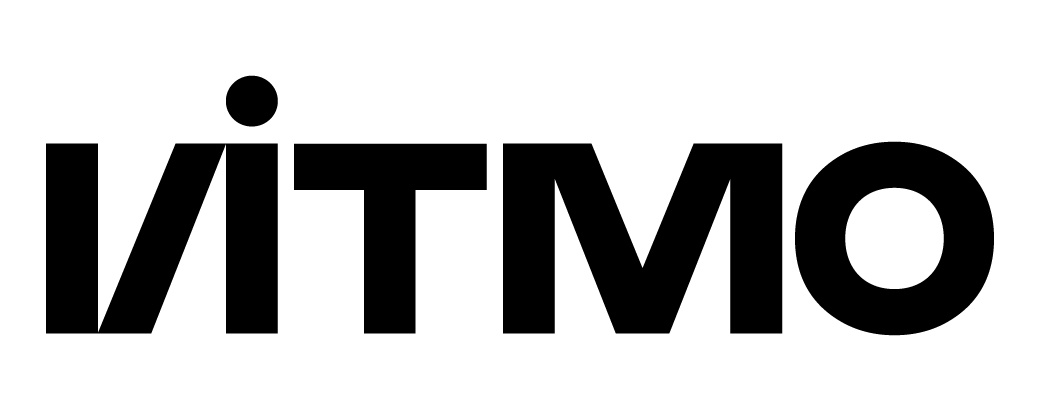
\includegraphics[width=\textwidth]{logo.png}
    % LAB INFO
    {
        \Large
        \textbf{Лабораторная работа по программированию №7}
        \par
        \normalsize
        \vspace*{0.75cm}
        \textbf{Вариант 310914}
        \par
    }
    \vfill
    % СREDITS
    \hfill\begin{minipage}{\dimexpr\textwidth-7.8cm}
        \textbf{Выполнил:}\par
        Степанов Арсений Алексеевич\par
        \vspace*{0.15cm}
        \textbf{Группа:}\par
        P3109\par
        \vspace*{0.15cm}
        \textbf{Преподаватель:}\par
        Наумова Надежда Александровна\par
    \end{minipage}
    \vfill
    Санкт-Петербург, \the\year{}г.
\end{titlepage}  
\section*{Цели}
Понять основы и разобраться в понятиях используемых при многопоточном программировании,
а также с основными методами аутентификации.
\section*{Задание}

\textbf{Доработать программу из лабораторной работы №6 следующим образом:}

\begin{enumerate}
    \item Организовать хранение коллекции в реляционной СУБД (PostgresQL). Убрать хранение коллекции в файле.
    \item Для генерации поля id использовать средства базы данных (sequence).
    \item Обновлять состояние коллекции в памяти только при успешном добавлении объекта в БД
    \item Все команды получения данных должны работать с коллекцией в памяти, а не в БД
    \item Организовать возможность регистрации и авторизации пользователей. У пользователя есть возможность указать пароль.
    \item Пароли при хранении хэшировать алгоритмом MD5
    \item Запретить выполнение команд не авторизованным пользователям.
    \item При хранении объектов сохранять информацию о пользователе, который создал этот объект.
    \item Пользователи должны иметь возможность просмотра всех объектов коллекции, но модифицировать могут только принадлежащие им.
    \item Для идентификации пользователя отправлять логин и пароль с каждым запросом.
\end{enumerate}
\textbf{Необходимо реализовать многопоточную обработку запросов.}
\begin{enumerate}
    \item Для многопоточного чтения запросов использовать ForkJoinPool
    \item Для многопотчной обработки полученного запроса использовать ForkJoinPool
    \item Для многопоточной отправки ответа использовать создание нового потока (java.lang.Thread)
    \item Для синхронизации доступа к коллекции использовать потокобезопасные аналоги коллекции из java.util.concurrent
\end{enumerate}
\section*{Код программы}
Исходный код расположен в \href{https://github.com/Armemius/ItmoStuff/tree/main/programming/lab7}{репозитории}.
\section*{Вывод}
В процессе доработки старой программы я познакомился с новыми концепциями, 
которые пригодятся мне в дальнейшей работе и обучении.
\end{document}